% Options for packages loaded elsewhere
\PassOptionsToPackage{unicode}{hyperref}
\PassOptionsToPackage{hyphens}{url}
%
\documentclass[
  ignorenonframetext,
]{beamer}
\usepackage{pgfpages}
\setbeamertemplate{caption}[numbered]
\setbeamertemplate{caption label separator}{: }
\setbeamercolor{caption name}{fg=normal text.fg}
\beamertemplatenavigationsymbolsempty
% Prevent slide breaks in the middle of a paragraph
\widowpenalties 1 10000
\raggedbottom
\setbeamertemplate{part page}{
  \centering
  \begin{beamercolorbox}[sep=16pt,center]{part title}
    \usebeamerfont{part title}\insertpart\par
  \end{beamercolorbox}
}
\setbeamertemplate{section page}{
  \centering
  \begin{beamercolorbox}[sep=12pt,center]{part title}
    \usebeamerfont{section title}\insertsection\par
  \end{beamercolorbox}
}
\setbeamertemplate{subsection page}{
  \centering
  \begin{beamercolorbox}[sep=8pt,center]{part title}
    \usebeamerfont{subsection title}\insertsubsection\par
  \end{beamercolorbox}
}
\AtBeginPart{
  \frame{\partpage}
}
\AtBeginSection{
  \ifbibliography
  \else
    \frame{\sectionpage}
  \fi
}
\AtBeginSubsection{
  \frame{\subsectionpage}
}
\usepackage{amsmath,amssymb}
\usepackage{iftex}
\ifPDFTeX
  \usepackage[T1]{fontenc}
  \usepackage[utf8]{inputenc}
  \usepackage{textcomp} % provide euro and other symbols
\else % if luatex or xetex
  \usepackage{unicode-math} % this also loads fontspec
  \defaultfontfeatures{Scale=MatchLowercase}
  \defaultfontfeatures[\rmfamily]{Ligatures=TeX,Scale=1}
\fi
\usepackage{lmodern}
\ifPDFTeX\else
  % xetex/luatex font selection
\fi
% Use upquote if available, for straight quotes in verbatim environments
\IfFileExists{upquote.sty}{\usepackage{upquote}}{}
\IfFileExists{microtype.sty}{% use microtype if available
  \usepackage[]{microtype}
  \UseMicrotypeSet[protrusion]{basicmath} % disable protrusion for tt fonts
}{}
\makeatletter
\@ifundefined{KOMAClassName}{% if non-KOMA class
  \IfFileExists{parskip.sty}{%
    \usepackage{parskip}
  }{% else
    \setlength{\parindent}{0pt}
    \setlength{\parskip}{6pt plus 2pt minus 1pt}}
}{% if KOMA class
  \KOMAoptions{parskip=half}}
\makeatother
\usepackage{xcolor}
\newif\ifbibliography
\usepackage{color}
\usepackage{fancyvrb}
\newcommand{\VerbBar}{|}
\newcommand{\VERB}{\Verb[commandchars=\\\{\}]}
\DefineVerbatimEnvironment{Highlighting}{Verbatim}{commandchars=\\\{\}}
% Add ',fontsize=\small' for more characters per line
\usepackage{framed}
\definecolor{shadecolor}{RGB}{248,248,248}
\newenvironment{Shaded}{\begin{snugshade}}{\end{snugshade}}
\newcommand{\AlertTok}[1]{\textcolor[rgb]{0.94,0.16,0.16}{#1}}
\newcommand{\AnnotationTok}[1]{\textcolor[rgb]{0.56,0.35,0.01}{\textbf{\textit{#1}}}}
\newcommand{\AttributeTok}[1]{\textcolor[rgb]{0.13,0.29,0.53}{#1}}
\newcommand{\BaseNTok}[1]{\textcolor[rgb]{0.00,0.00,0.81}{#1}}
\newcommand{\BuiltInTok}[1]{#1}
\newcommand{\CharTok}[1]{\textcolor[rgb]{0.31,0.60,0.02}{#1}}
\newcommand{\CommentTok}[1]{\textcolor[rgb]{0.56,0.35,0.01}{\textit{#1}}}
\newcommand{\CommentVarTok}[1]{\textcolor[rgb]{0.56,0.35,0.01}{\textbf{\textit{#1}}}}
\newcommand{\ConstantTok}[1]{\textcolor[rgb]{0.56,0.35,0.01}{#1}}
\newcommand{\ControlFlowTok}[1]{\textcolor[rgb]{0.13,0.29,0.53}{\textbf{#1}}}
\newcommand{\DataTypeTok}[1]{\textcolor[rgb]{0.13,0.29,0.53}{#1}}
\newcommand{\DecValTok}[1]{\textcolor[rgb]{0.00,0.00,0.81}{#1}}
\newcommand{\DocumentationTok}[1]{\textcolor[rgb]{0.56,0.35,0.01}{\textbf{\textit{#1}}}}
\newcommand{\ErrorTok}[1]{\textcolor[rgb]{0.64,0.00,0.00}{\textbf{#1}}}
\newcommand{\ExtensionTok}[1]{#1}
\newcommand{\FloatTok}[1]{\textcolor[rgb]{0.00,0.00,0.81}{#1}}
\newcommand{\FunctionTok}[1]{\textcolor[rgb]{0.13,0.29,0.53}{\textbf{#1}}}
\newcommand{\ImportTok}[1]{#1}
\newcommand{\InformationTok}[1]{\textcolor[rgb]{0.56,0.35,0.01}{\textbf{\textit{#1}}}}
\newcommand{\KeywordTok}[1]{\textcolor[rgb]{0.13,0.29,0.53}{\textbf{#1}}}
\newcommand{\NormalTok}[1]{#1}
\newcommand{\OperatorTok}[1]{\textcolor[rgb]{0.81,0.36,0.00}{\textbf{#1}}}
\newcommand{\OtherTok}[1]{\textcolor[rgb]{0.56,0.35,0.01}{#1}}
\newcommand{\PreprocessorTok}[1]{\textcolor[rgb]{0.56,0.35,0.01}{\textit{#1}}}
\newcommand{\RegionMarkerTok}[1]{#1}
\newcommand{\SpecialCharTok}[1]{\textcolor[rgb]{0.81,0.36,0.00}{\textbf{#1}}}
\newcommand{\SpecialStringTok}[1]{\textcolor[rgb]{0.31,0.60,0.02}{#1}}
\newcommand{\StringTok}[1]{\textcolor[rgb]{0.31,0.60,0.02}{#1}}
\newcommand{\VariableTok}[1]{\textcolor[rgb]{0.00,0.00,0.00}{#1}}
\newcommand{\VerbatimStringTok}[1]{\textcolor[rgb]{0.31,0.60,0.02}{#1}}
\newcommand{\WarningTok}[1]{\textcolor[rgb]{0.56,0.35,0.01}{\textbf{\textit{#1}}}}
\usepackage{longtable,booktabs,array}
\usepackage{calc} % for calculating minipage widths
\usepackage{caption}
% Make caption package work with longtable
\makeatletter
\def\fnum@table{\tablename~\thetable}
\makeatother
\usepackage{graphicx}
\makeatletter
\def\maxwidth{\ifdim\Gin@nat@width>\linewidth\linewidth\else\Gin@nat@width\fi}
\def\maxheight{\ifdim\Gin@nat@height>\textheight\textheight\else\Gin@nat@height\fi}
\makeatother
% Scale images if necessary, so that they will not overflow the page
% margins by default, and it is still possible to overwrite the defaults
% using explicit options in \includegraphics[width, height, ...]{}
\setkeys{Gin}{width=\maxwidth,height=\maxheight,keepaspectratio}
% Set default figure placement to htbp
\makeatletter
\def\fps@figure{htbp}
\makeatother
\setlength{\emergencystretch}{3em} % prevent overfull lines
\providecommand{\tightlist}{%
  \setlength{\itemsep}{0pt}\setlength{\parskip}{0pt}}
\setcounter{secnumdepth}{-\maxdimen} % remove section numbering
\ifLuaTeX
  \usepackage{selnolig}  % disable illegal ligatures
\fi
\IfFileExists{bookmark.sty}{\usepackage{bookmark}}{\usepackage{hyperref}}
\IfFileExists{xurl.sty}{\usepackage{xurl}}{} % add URL line breaks if available
\urlstyle{same}
\hypersetup{
  pdftitle={TMA4315 Generalized linear models H2018},
  pdfauthor={Mette Langaas, Department of Mathematical Sciences, NTNU, with contibutions from Ingeborg G. Hem},
  hidelinks,
  pdfcreator={LaTeX via pandoc}}

\title{TMA4315 Generalized linear models H2018}
\subtitle{Module 6: Categorical regression}
\author{Mette Langaas, Department of Mathematical Sciences, NTNU, with
contibutions from Ingeborg G. Hem}
\date{25.10.2017 {[}PL{]}, 26.10.2017 {[}IL{]}}

\begin{document}
\frame{\titlepage}

\begin{frame}
(Latest changes: 24.10: added IL + corrected typos, 23.10.2018: first
version)
\end{frame}

\begin{frame}{Overview}
\protect\hypertarget{overview}{}
\begin{block}{Learning material}
\protect\hypertarget{learning-material}{}
This topic is \emph{new} on the reading list this year.

\begin{itemize}
\tightlist
\item
  Textbook: Fahrmeir et al (2013): Chapter 6 (not p 344-345 nominal
  models and latent utility models, not 6.3.2 Sequential model, and not
  category specific varables on page 344-3458).
\item
  \href{https://www.math.ntnu.no/emner/TMA4315/2018h/M62018.pdf}{Classnotes
  25.10.2018}
\end{itemize}
\end{block}
\end{frame}

\begin{frame}
\begin{block}{Topics}
\protect\hypertarget{topics}{}
\begin{itemize}
\item
  multinomial random component
\item
  nominal vs.~ordinal response
\item
  ungrouped and grouped data
\item
  multivariate exponential family
\item
  nominal response and logit models
\item
  ordinal reponse and logit models - based on a latent model
\item
  likelihood inference
\end{itemize}

Jump to \protect\hyperlink{interactive}{interactive}.
\end{block}
\end{frame}

\begin{frame}{Categorical random component}
\protect\hypertarget{categorical-random-component}{}
We consider a situation where our random variable (response) is given as
one of \(c+1\) possible categories (where we will look at category
\(c+1\) as the reference category).

The categories will either be

\begin{itemize}
\tightlist
\item
  Unordered: \emph{nominal response variable}. Example: food types in
  alligator example.
\item
  Ordered: \emph{ordered response variable}. Example: degrees of mental
  impairment.
\end{itemize}
\end{frame}

\begin{frame}
Assumptions:

\begin{itemize}
\tightlist
\item
  \emph{Independent} observation pairs \(({\bf Y}_i,{\bf x}_i)\).
\item
  \(\pi_{ir}\): probability that the response is category \(r\) for
  subject \(i\).
\item
  \(\sum_{s=1}^{c+1}\pi_{is}=1\) for all \(i\), so that
  \(\pi_{i,c+1}=1-\sum_{s=1}^{c}\pi_{is}\). So, we have \(c\)
  probabilities to estimate.
\item
  Further, the covariate vector \({\bf x}_i\) consists of the same
  measurements for each response category (that is, not different
  covariate types that are measured for each response category - which
  in our textbook is written as \emph{independent of the response
  category}).
\end{itemize}
\end{frame}

\begin{frame}
When coding the response variable we use a dummy variable coding with
\(c\) elements (the \(c+1\) category is the reference level). This means
that if we have that \(\pi_{ir}=1\) then
\({\bf y}_i=(0,0,\ldots,0,1,0,\ldots,0)\) with a value of \(1\) in the
\(r\)th element of \({\bf y}_i\). If observation \(i\) comes from
category \(c+1\) we have \({\bf y}_i=(0,0,\ldots,0)\).
\end{frame}

\begin{frame}
\begin{block}{Categorical regression}
\protect\hypertarget{categorical-regression}{}
is modelling and estimating the probabilites
\(\pi_{ir}=P(Y_i=r)=P(Y_{ir}=1)\) as a function of the covariates
\({\bf x}_i\). The modelling is done differently for nominal (unordered)
and ordered categories, but both rely upon the multinomial distribution.

For unordered categories, a Poisson distribution can also be used
\end{block}
\end{frame}

\begin{frame}
\begin{block}{The multinomial distribution}
\protect\hypertarget{the-multinomial-distribution}{}
Probability mass function for one observation:

\[f({\bf y})=\pi_1^{y_{1}} \pi_2^{y_{2}} \cdots \pi_c^{y_c} (1-\pi_1-\pi_2-\cdots-\pi_c)^{1-y_1-y_2-\cdots-y_c}\]
where then \({\bf y}=(y_1,y_2,\ldots,y_c)\) and \(y_r=1\) if the
observation comes from the \(r\)th category.
\end{block}
\end{frame}

\begin{frame}
If we then have \(m\) independent trials then
\({\bf y}=(y_1,y_2,\ldots,y_c)\) is summed over our \(m\) responses, so
that \(y_r\) is the number of observations where the response is from
the \(r\)th category.

\[f({\bf y})=\frac{m!}{y_1!\cdots y_c! (m-y_1-\cdots -y_c)!}\pi_1^{y_{1}} \pi_2^{y_{2}} \cdots \pi_c^{y_c}(1-\pi_1-\pi_2-\cdots-\pi_c)^{m-y_1-y_2-\cdots-y_c}\]
\end{frame}

\begin{frame}
The mean and the covariance matrix of the random vector \({\bf Y}\) are
given by:

\[\text{E}({\bf Y})=m\boldsymbol{\pi}=\begin{pmatrix}m\pi_1\\m\pi_2\\ \vdots \\ m\pi_c\end{pmatrix}\]
\[\text{Cov}({\bf Y})=m \begin{pmatrix}\pi_1(1-\pi_1)& -\pi_1\pi_2&\cdots &-\pi_1\pi_c\\
-\pi_2\pi_1& \pi_2(1-\pi_2)&\cdots &-\pi_2\pi_c\\
\vdots & \vdots & \ddots & \vdots\\
-\pi_c\pi_1& -\pi_c\pi_2&\cdots & \pi_c(1-\pi_c)\end{pmatrix}\]

\textbf{Q}: what about \(\text{E}(Y_{c+1})\) and
\(\text{Cov}(Y_1,Y_{c+1})\)?
\end{frame}

\begin{frame}
Finally, if we look at \(\bar{Y}_r=\frac{1}{m}Y_r\) then
\(\bar{\bf Y}=\frac{1}{m}{\bf Y}\) follows a scaled multinomial
distribution \(\bar{\bf Y}\sim \frac{1}{m}M(m,{\boldsymbol \pi})\) with
\(\text{E}(\bar{\bf Y})={\boldsymbol \pi}\) and
\(\text{Cov}(\bar{\bf Y})=\frac{1}{m^2}\text{Cov}({\bf Y})\).
\end{frame}

\begin{frame}{Data}
\protect\hypertarget{data}{}
\begin{block}{Ungrouped data}
\protect\hypertarget{ungrouped-data}{}
\[{\bf Y}=\begin{pmatrix} Y_{11}& Y_{12} & \cdots & Y_{1c}\\
Y_{21}& Y_{22} & \cdots & Y_{2c}\\
\vdots & \vdots & \ddots & \vdots\\
Y_{n1}& Y_{n2} & \cdots & Y_{nc}\\
\end{pmatrix}\]

and \({\bf X}\) is an \(n \times p\) matrix as usual.
\end{block}
\end{frame}

\begin{frame}
\begin{block}{Grouped data}
\protect\hypertarget{grouped-data}{}
As for the binomial case we look at the number of occurences with a
group - that is, one covariate pattern.

\[{\bf Y}=\begin{pmatrix} Y_{11}& Y_{12} & \cdots & Y_{1c}\\
Y_{21}& Y_{22} & \cdots & Y_{2c}\\
\vdots & \vdots & \ddots & \vdots\\
Y_{G1}& Y_{G2} & \cdots & Y_{Gc}\\
\end{pmatrix}\]

The notation here is that we have \(n_i\) observation for each covariate
pattern (group) \(i\) for \(i=1,\ldots,G\). This will replace the \(m\)
used for the multinomial distribution above.
\end{block}
\end{frame}

\begin{frame}{Regression with nominal responses}
\protect\hypertarget{regression-with-nominal-responses}{}
nominal=unordered

Agresti (2015, p203): ``The model treats the response variable as
nominal scale in the following sense: if the model holds and the outcome
categories are permuted in any way, the model still holds with the
corresponding permuatation of the effects.''
\end{frame}

\begin{frame}
This is a generalization of the binary logit model with \(P(Y=1)\) vs
\(P(Y=0)\), to \(c\) models of \(\pi_{ir}\) vs \(\pi_{i,c+1}\) for
\(r=1,\ldots,c\).

The models can be written using log ratios:
\[ \ln(\frac{\pi_{ir}}{\pi_{i,c+1}})={\bf x}_i^T {\boldsymbol \beta}_r\]

Remark: \({\boldsymbol \beta}_r\) is the \(p\times 1\) coefficient
vector for the \(r\)th response

Using this we may also look at the log ratio for any two probabilites
\(\pi_{ia}\) and \(\pi_{ib}\):

\[\ln(\frac{\pi_{ia}}{\pi_{ib}})=\ln(\frac{\pi_{ia}}{\pi_{i,c+1}})-\ln(\frac{\pi_{ib}}{\pi_{i,c+1}})={\bf x}_i^T ({\boldsymbol \beta}_a-{\boldsymbol \beta}_b)\]
\end{frame}

\begin{frame}
Alternatively, we may write out the model for the probabilites:

\[P(Y_i=r)=\pi_{ir}=\frac{\exp({\bf x}_i^T {\boldsymbol\beta}_r)}{1+\sum_{s=1}^{c}\exp({\bf x}_i^T {\boldsymbol\beta}_s)}\]

\[P(Y_i=c+1)=\pi_{i,c+1}=1-\pi_{i1}-\cdots \pi_{ic}=\frac{1}{1+\sum_{s=1}^{c}\exp({\bf x}_i^T {\boldsymbol\beta}_s)}\]
\end{frame}

\begin{frame}
\begin{block}{Multivariate GLM}
\protect\hypertarget{multivariate-glm}{}
This is a multivariate GLM and the multinomial distribution is \emph{a
multivariate exponential family}.

\[f({\bf y}_i,{\boldsymbol \theta}_i,\phi)=\exp(\frac{{\bf y}_i^T{\boldsymbol \theta}_i-b({\boldsymbol \theta}_i)w_i}{\phi}+c({\bf y}_i,\phi,w_i))\]

where \({\boldsymbol \theta}\) has dimension \(c\).
\end{block}
\end{frame}

\begin{frame}
\begin{block}{Multivariate GLM-set-up}
\protect\hypertarget{multivariate-glm-set-up}{}
\begin{enumerate}
\tightlist
\item
  \({\bf Y}_i\) is multinomial with
\end{enumerate}

\[{\boldsymbol \mu}_i=\text{E}({\bf Y}_i)=
{\boldsymbol \pi}_i=\begin{pmatrix} \pi_{i1}\\ \pi_{i2}\\ \vdots \\ \pi_{i,c+1}\end{pmatrix}\]
Remark: if grouped data we instead look at
\(\bar{\bf Y}_i\sim \frac{1}{n_i}M(n_i,\pi_i)\) so that the mean is
\({\boldsymbol \pi}_i\)
\end{block}
\end{frame}

\begin{frame}
\begin{enumerate}
\setcounter{enumi}{1}
\tightlist
\item
  Linear predictor is now a \(c \times 1\) vector:
\end{enumerate}

\[{\boldsymbol \eta}_i=\begin{pmatrix} \eta_{i1}\\ \eta_{i2}\\ \vdots \\ \eta_{i,c}\end{pmatrix}=
\begin{pmatrix} {\bf x}_i^T{\boldsymbol \beta}_{1}\\ {\bf x}_i^T{\boldsymbol \beta}_{2}\\ \vdots \\ {\bf x}_i^T{\boldsymbol \beta}_{c} \end{pmatrix}\]
\end{frame}

\begin{frame}
\begin{enumerate}
\setcounter{enumi}{2}
\tightlist
\item
  Link functions (\(c\) of those):
  \({\bf g}(\boldsymbol{\mu}_i)={\boldsymbol \eta}_i\) where for the
  \emph{nominal logit data model} element \(r\) (for \(r=1,\ldots, c\))
  of \({\bf g}\) is
\end{enumerate}

\[ g_{r}(\boldsymbol{\mu}_i)=\ln(\frac{\mu_{ir}}{1-\mu_{i1}-\cdots-\mu_{ic}})=
\ln(\frac{\pi_{ir}}{1-\pi_{i1}-\cdots-\pi_{ic}})\]

We also define response functions \((\bf h)\) with elements \(h_r\)
given by \(\pi_{ir}=h_r(\eta_{i1},\eta_{i2},\ldots,\eta_{ic})\), and we
have for the \emph{nominal data model}

\[\pi_{ir}=h_r((\eta_{i1},\eta_{i2},\ldots,\eta_{ic})=\frac{\exp(\eta_{ir})}{1+\sum_{s=1}^c \exp(\eta_{is})}\]
\end{frame}

\begin{frame}
It turns out that the reference category logits are the canonical links
for the multinomial distribution GLM.

In this case, as for the univariate exponential family GLM the
loglikelihood is concave with an unique maximum (if it exists) and the
expected and observed Fisher information matrices are equal.

As before, we find maximum likelihood parameter estimates from the
Fisher scoring or Newton Raphson method.

Remember: now we have \(p\times c\) parameters to estimate --- \(p\) for
each category \(c\). All of these coefficients may either be put into a
long vector (length \(p\cdot c\)) --- which might be easiest to
understand for the estimation, or into a matrix of dimension
\(p \times c\) --- might be easier for viewing.
\end{frame}

\begin{frame}
\begin{block}{Likelihood}
\protect\hypertarget{likelihood}{}
(grouped data)

With the notation that \({\boldsymbol \beta}\) is a long vector with the
coefficients for the \(c\) categories stacked upon eachother.

\[L({\boldsymbol \beta})=\Pi_{i=1}^G f({\bf y}_i\mid {\boldsymbol \pi})\]
where \(f\) is the multinomial distribution function.
\end{block}
\end{frame}

\begin{frame}
\begin{block}{Loglikelihood}
\protect\hypertarget{loglikelihood}{}
\[ l({\boldsymbol \beta})\propto\sum_{i=1}^G \sum_{s=1}^{c+1} y_{is}\ln(\pi_{is})\]

where we remember that \(y_{i,c+1}=n_i-y_{i1}-\cdots-y_{ic}\), and
\(1-\pi_{i1}-\cdots \pi_{ic}\).

(This formula is also correct for the ordinal model of the next
section.) General formulas for the score function and expected Fisher
information matrix follow later.
\end{block}
\end{frame}

\begin{frame}
\begin{block}{Deviance}
\protect\hypertarget{deviance}{}
The derivation used for the binary GLM model generalizes directly ot the
multinomial GLM. The fitted probabilities are \(\hat\pi_{ij}\) (group
\(i\) and category \(j\)) and the saturated model (grouped data) is
\(n_i \tilde\pi_{ij}=y_{ij}\).
\[D=2 \sum_{i=1}^G \sum_{s=1}^{c+1} y_{is}\ln(\frac{{y}_{is}}{n_i \hat{\pi}_{is}})\]

The asymptotic distribution is as before \(\chi^2\) with ``the number of
groups times number of categories minus 1 (Gc)'' minus ``the number of
covariates (cp)'', giving \(Gc-cp=c(G-p)\) degrees of freedom.
\end{block}
\end{frame}

\begin{frame}
The deviance can be used for model check with grouped data (\(G\) groups
with \(n_i\) observations), but can be used to compare nested
unsaturated models also for individual (ungrouped) data, with again an
asymptotic \(\chi^2\) distribution with the difference of number of
parameters between the two models.

This formula is also correct for the ordinal model of the next section,
except that the number of parameters estimated differ.
\end{frame}

\begin{frame}
\begin{block}{Alligators example}
\protect\hypertarget{alligators-example}{}
Example and data are taken from Agresti (2015, pages 217-219).

Research question: what is the factors influencing the primary food
choice of alligators?

Data are from 219 captured alligators from four lakes in Florida, where
the stomack contents of the alligators were investigated. The weight of
different types of food was measured, and then the primary food choice
(highest weight) was noted. The primary choice is given as y1:y5 below.
In addition the size of the alligator (non-adult or adult) was
registered.
\end{block}
\end{frame}

\begin{frame}
\begin{itemize}
\tightlist
\item
  lake: each of the 4 lakes in Florida (1:4)
\item
  size: non-adult=the size of the alligator (0: 2.3 meters or smaller)
  and adult=(1: larger than 2.3 meters)
\item
  y1: fish
\item
  y2: inverterbrate
\item
  y3: reptile
\item
  y4: bird
\item
  y5: other
\end{itemize}

These data are grouped, and we let y1:fish be the reference category.
\end{frame}

\begin{frame}[fragile]
\small

\begin{Shaded}
\begin{Highlighting}[]
\CommentTok{\# data from Agresti (2015), section 6, with use of the VGAM packages}
\NormalTok{data }\OtherTok{=} \StringTok{"http://www.stat.ufl.edu/\textasciitilde{}aa/glm/data/Alligators.dat"}
\NormalTok{ali }\OtherTok{=} \FunctionTok{read.table}\NormalTok{(data, }\AttributeTok{header =}\NormalTok{ T)}
\NormalTok{ali}
\FunctionTok{attach}\NormalTok{(ali)}
\end{Highlighting}
\end{Shaded}

\begin{verbatim}
##   lake size y1 y2 y3 y4 y5
## 1    1    1 23  4  2  2  8
## 2    1    0  7  0  1  3  5
## 3    2    1  5 11  1  0  3
## 4    2    0 13  8  6  1  0
## 5    3    1  5 11  2  1  5
## 6    3    0  8  7  6  3  5
## 7    4    1 16 19  1  2  3
## 8    4    0 17  1  0  1  3
\end{verbatim}
\end{frame}

\begin{frame}[fragile]
\begin{Shaded}
\begin{Highlighting}[]
\NormalTok{y.data }\OtherTok{=} \FunctionTok{cbind}\NormalTok{(y2, y3, y4, y5, y1)}
\NormalTok{y.data}
\FunctionTok{dim}\NormalTok{(y.data)}
\NormalTok{x.data }\OtherTok{=} \FunctionTok{model.matrix}\NormalTok{(}\SpecialCharTok{\textasciitilde{}}\NormalTok{size }\SpecialCharTok{+} \FunctionTok{factor}\NormalTok{(lake), }\AttributeTok{data =}\NormalTok{ ali)}
\NormalTok{x.data}
\FunctionTok{dim}\NormalTok{(x.data)}
\end{Highlighting}
\end{Shaded}

\begin{verbatim}
##      y2 y3 y4 y5 y1
## [1,]  4  2  2  8 23
## [2,]  0  1  3  5  7
## [3,] 11  1  0  3  5
## [4,]  8  6  1  0 13
## [5,] 11  2  1  5  5
## [6,]  7  6  3  5  8
## [7,] 19  1  2  3 16
## [8,]  1  0  1  3 17
## [1] 8 5
##   (Intercept) size factor(lake)2 factor(lake)3 factor(lake)4
## 1           1    1             0             0             0
## 2           1    0             0             0             0
## 3           1    1             1             0             0
## 4           1    0             1             0             0
## 5           1    1             0             1             0
## 6           1    0             0             1             0
## 7           1    1             0             0             1
## 8           1    0             0             0             1
## attr(,"assign")
## [1] 0 1 2 2 2
## attr(,"contrasts")
## attr(,"contrasts")$`factor(lake)`
## [1] "contr.treatment"
## 
## [1] 8 5
\end{verbatim}
\end{frame}

\begin{frame}[fragile]
\begin{Shaded}
\begin{Highlighting}[]
\CommentTok{\# We use library VGAM:}
\FunctionTok{library}\NormalTok{(VGAM)}

\CommentTok{\# We fit a multinomial logit model with fish (y1) as the reference category:}
\NormalTok{fit.main }\OtherTok{=} \FunctionTok{vglm}\NormalTok{(}\FunctionTok{cbind}\NormalTok{(y2, y3, y4, y5, y1) }\SpecialCharTok{\textasciitilde{}}\NormalTok{ size }\SpecialCharTok{+} \FunctionTok{factor}\NormalTok{(lake), }\AttributeTok{family =}\NormalTok{ multinomial,}
    \AttributeTok{data =}\NormalTok{ ali)}
\CommentTok{\# summary(fit.main)}
\FunctionTok{pchisq}\NormalTok{(}\FunctionTok{deviance}\NormalTok{(fit.main), }\FunctionTok{df.residual}\NormalTok{(fit.main), }\AttributeTok{lower.tail =} \ConstantTok{FALSE}\NormalTok{)}
\end{Highlighting}
\end{Shaded}

\begin{verbatim}
## [1] 0.1466189
\end{verbatim}
\end{frame}

\begin{frame}[fragile]
\normalsize

\textbf{Q}:

\begin{itemize}
\tightlist
\item
  Why is the number of degrees of freedom for the residual deviance 12?
  Hint: there are 8 covariate patterns, and we have 5 reponse
  categories.
\item
  How can you interpret the coefficient for inverterbrate (y2) and size?
  Hint: we have y2,y3,y4,y5 as 1:4.
\end{itemize}

\small

\begin{Shaded}
\begin{Highlighting}[]
\FunctionTok{exp}\NormalTok{(}\FunctionTok{coefficients}\NormalTok{(fit.main))}
\end{Highlighting}
\end{Shaded}

\begin{verbatim}
##   (Intercept):1   (Intercept):2   (Intercept):3   (Intercept):4          size:1 
##       0.0404626       0.1259644       0.2471007       0.3402497       4.2982356 
##          size:2          size:3          size:4 factor(lake)2:1 factor(lake)2:2 
##       0.7037987       0.5322405       1.3931262      13.4043318       3.3739877 
## factor(lake)2:3 factor(lake)2:4 factor(lake)3:1 factor(lake)3:2 factor(lake)3:3 
##       0.2596748       0.4401925      16.1245576       5.4329197       1.4808988 
## factor(lake)3:4 factor(lake)4:1 factor(lake)4:2 factor(lake)4:3 factor(lake)4:4 
##       1.9940595       5.2506853       0.2885818       0.4990158       0.4377111
\end{verbatim}

\normalsize
\end{frame}

\begin{frame}[fragile]
Testing out other models, and comparing with LRT-test - by using
deviances for different models.

\begin{Shaded}
\begin{Highlighting}[]
\CommentTok{\# Fit model with only lake:}
\NormalTok{fit.lake }\OtherTok{=} \FunctionTok{vglm}\NormalTok{(}\FunctionTok{cbind}\NormalTok{(y2, y3, y4, y5, y1) }\SpecialCharTok{\textasciitilde{}} \FunctionTok{factor}\NormalTok{(lake), }\AttributeTok{family =}\NormalTok{ multinomial, }\AttributeTok{data =}\NormalTok{ ali)}
\CommentTok{\# Test effect of size (no anova command is available)}
\NormalTok{(}\AttributeTok{G2 =} \FunctionTok{deviance}\NormalTok{(fit.lake) }\SpecialCharTok{{-}} \FunctionTok{deviance}\NormalTok{(fit.main))}
\NormalTok{(}\AttributeTok{df.diff =} \FunctionTok{df.residual}\NormalTok{(fit.lake) }\SpecialCharTok{{-}} \FunctionTok{df.residual}\NormalTok{(fit.main))}
\DecValTok{1} \SpecialCharTok{{-}} \FunctionTok{pchisq}\NormalTok{(G2, df.diff)}
\CommentTok{\# Size has a significant effect}
\end{Highlighting}
\end{Shaded}

\begin{verbatim}
## [1] 21.08741
## [1] 4
## [1] 0.0003042796
\end{verbatim}
\end{frame}

\begin{frame}[fragile]
\begin{Shaded}
\begin{Highlighting}[]
\CommentTok{\# Fit model with only size:}
\NormalTok{fit.size }\OtherTok{=} \FunctionTok{vglm}\NormalTok{(}\FunctionTok{cbind}\NormalTok{(y2, y3, y4, y5, y1) }\SpecialCharTok{\textasciitilde{}}\NormalTok{ size, }\AttributeTok{family =}\NormalTok{ multinomial, }\AttributeTok{data =}\NormalTok{ ali)}

\CommentTok{\# Test effect of lake}
\NormalTok{(}\AttributeTok{G2 =} \FunctionTok{deviance}\NormalTok{(fit.size) }\SpecialCharTok{{-}} \FunctionTok{deviance}\NormalTok{(fit.main))}
\NormalTok{(}\AttributeTok{df.diff =} \FunctionTok{df.residual}\NormalTok{(fit.size) }\SpecialCharTok{{-}} \FunctionTok{df.residual}\NormalTok{(fit.main))}
\DecValTok{1} \SpecialCharTok{{-}} \FunctionTok{pchisq}\NormalTok{(G2, df.diff)}
\CommentTok{\# Lake has a significant effect}
\end{Highlighting}
\end{Shaded}

\begin{verbatim}
## [1] 49.13308
## [1] 12
## [1] 1.982524e-06
\end{verbatim}
\end{frame}

\begin{frame}[fragile]
\textbf{Q}: explain what is presented below, in particular ``what is the
probability that the main food source is fish given size=0 and lake=1''?

\small

\begin{Shaded}
\begin{Highlighting}[]
\FunctionTok{library}\NormalTok{(knitr)}
\CommentTok{\# Fitted values for main effect model \textquotesingle{}fit.main\textquotesingle{}:}
\NormalTok{fitted }\OtherTok{=} \FunctionTok{data.frame}\NormalTok{(}\FunctionTok{fitted}\NormalTok{(fit.main), }\AttributeTok{lake =}\NormalTok{ ali}\SpecialCharTok{$}\NormalTok{lake, }\AttributeTok{size =}\NormalTok{ ali}\SpecialCharTok{$}\NormalTok{size)}
\FunctionTok{kable}\NormalTok{(fitted)}
\end{Highlighting}
\end{Shaded}

\begin{longtable}[]{@{}rrrrrrr@{}}
\toprule\noalign{}
y2 & y3 & y4 & y5 & y1 & lake & size \\
\midrule\noalign{}
\endhead
0.0930988 & 0.0474566 & 0.0704015 & 0.2537396 & 0.5353035 & 1 & 1 \\
0.0230717 & 0.0718246 & 0.1408963 & 0.1940096 & 0.5701978 & 1 & 0 \\
0.6018967 & 0.0772276 & 0.0088175 & 0.0538721 & 0.2581861 & 2 & 1 \\
0.2486452 & 0.1948374 & 0.0294161 & 0.0686628 & 0.4584385 & 2 & 0 \\
0.5168385 & 0.0887672 & 0.0358947 & 0.1742005 & 0.1842990 & 3 & 1 \\
0.1929612 & 0.2023995 & 0.1082251 & 0.2006616 & 0.2957525 & 3 & 0 \\
0.4128558 & 0.0115665 & 0.0296712 & 0.0938024 & 0.4521040 & 4 & 1 \\
0.1396778 & 0.0238987 & 0.0810674 & 0.0979136 & 0.6574425 & 4 & 0 \\
\bottomrule\noalign{}
\end{longtable}

\normalsize

\normalsize
\end{frame}

\begin{frame}{Regression with ordinal responses}
\protect\hypertarget{regression-with-ordinal-responses}{}
(we will only consider cumulative models - and not sequential models)

An unobservable latent variable \(U_i\) drives the observed category
\(Y_i\).

\[ Y_i=r \Leftrightarrow \theta_{r-1}\le U_i \le \theta_r\] where these
\(\theta\)s are our unobservable thresholds, and the thresholds are
monotonely increasing,
\(-\infty=\theta_0< \theta_1 < \cdots < \theta_{c+1}=\infty\).

We further assume that the latent variables are dependent on our
covariates through

\[ U_i=-{\bf x}_i^T{\boldsymbol \beta} + \varepsilon_i\]

where we have a new random variable that has cumulative distribution
function (cdf) \(F\). No intercept is included due to identifiability
issuse (shift in intercept would produce the same effect as negative
shift in threshold).
\end{frame}

\begin{frame}
We get rid of the latent variable \(U_i\) by considereing

\[P(Y_i\le r)=P(U_i\le \theta_r)=P(-{\bf x}_i^T {\boldsymbol \beta}+\varepsilon_i \le \theta_r)\]
\[=P(\varepsilon_i \le \theta_r+{\bf x}_i^T {\boldsymbol \beta})=F(\theta_r+{\bf x}_i^T {\boldsymbol \beta}) \]

Observe that the final expression does not include the latent variable
\(U_i\), but includes the unknown threshold and \(k\) regression
parameters.
\end{frame}

\begin{frame}
Different choices of \(F\) will give different models, and we will only
consider \(F\) to be the cdf for the logistic distribution. (Another
popular choice is the cdf of the standard normal distribution.)

\[P(Y_i\le r)=\frac{\exp(\theta_r+{\bf x}_i^T {\boldsymbol \beta})}{1+\exp(\theta_r+{\bf x}_i^T {\boldsymbol \beta})}\]

which also can be written as

\[ \ln(\frac{P(Y_i\le r)}{P(Y_i> r)})=\theta_r+{\bf x}_i^T {\boldsymbol \beta}\]
\end{frame}

\begin{frame}
Our model is a proportional odds model, in the sense that the cumulative
odds are proportional across categories

\[\frac{\frac{P(Y\le r\mid {\bf x}_i)}{P(Y> r\mid {\bf x}_i)}}
{\frac{P(Y\le r\mid {\bf x}^*_i)}{P(Y> r\mid {\bf x}^*_i)}}= \exp(({\bf x}_i-{\bf x}^*_i)^T {\boldsymbol \beta})\]

Observe that this is independent of \(r\).
\end{frame}

\begin{frame}
\begin{block}{Response function}
\protect\hypertarget{response-function}{}
What is the response function here?

\[\pi_{i1}=F(\eta_{i1})\] \[\pi_{ir}=F(\eta_{ir})-F(\eta_{i,r-1})\]

where \(\eta_{ir}=\theta_r+{\bf x}_i^T{\boldsymbol \beta}\), and \(F\)
is the logistic cdf.
\end{block}
\end{frame}

\begin{frame}
\begin{block}{Plotting the cumulative probabilites}
\protect\hypertarget{plotting-the-cumulative-probabilites}{}
We have five categories, where the fifth is the reference category.

True parameters

\begin{itemize}
\tightlist
\item
  \(\theta_1=0\), \(\theta_2=1\), \(\theta_3=4\) and \(\theta_4=6\) and
\item
  one covariate with parameter \(\beta=1\).
\end{itemize}

The graph shows the cumulative probability \(P(Y\le r)\) for \(r=1\)
(red), \(r=2\) (organge), \(r=3\) (green), \(r=4\) (purple).

Observe the parallell lines.

What would \(P(Y\le 5)\) be? Why is this missing from the plot?
\end{block}
\end{frame}

\begin{frame}
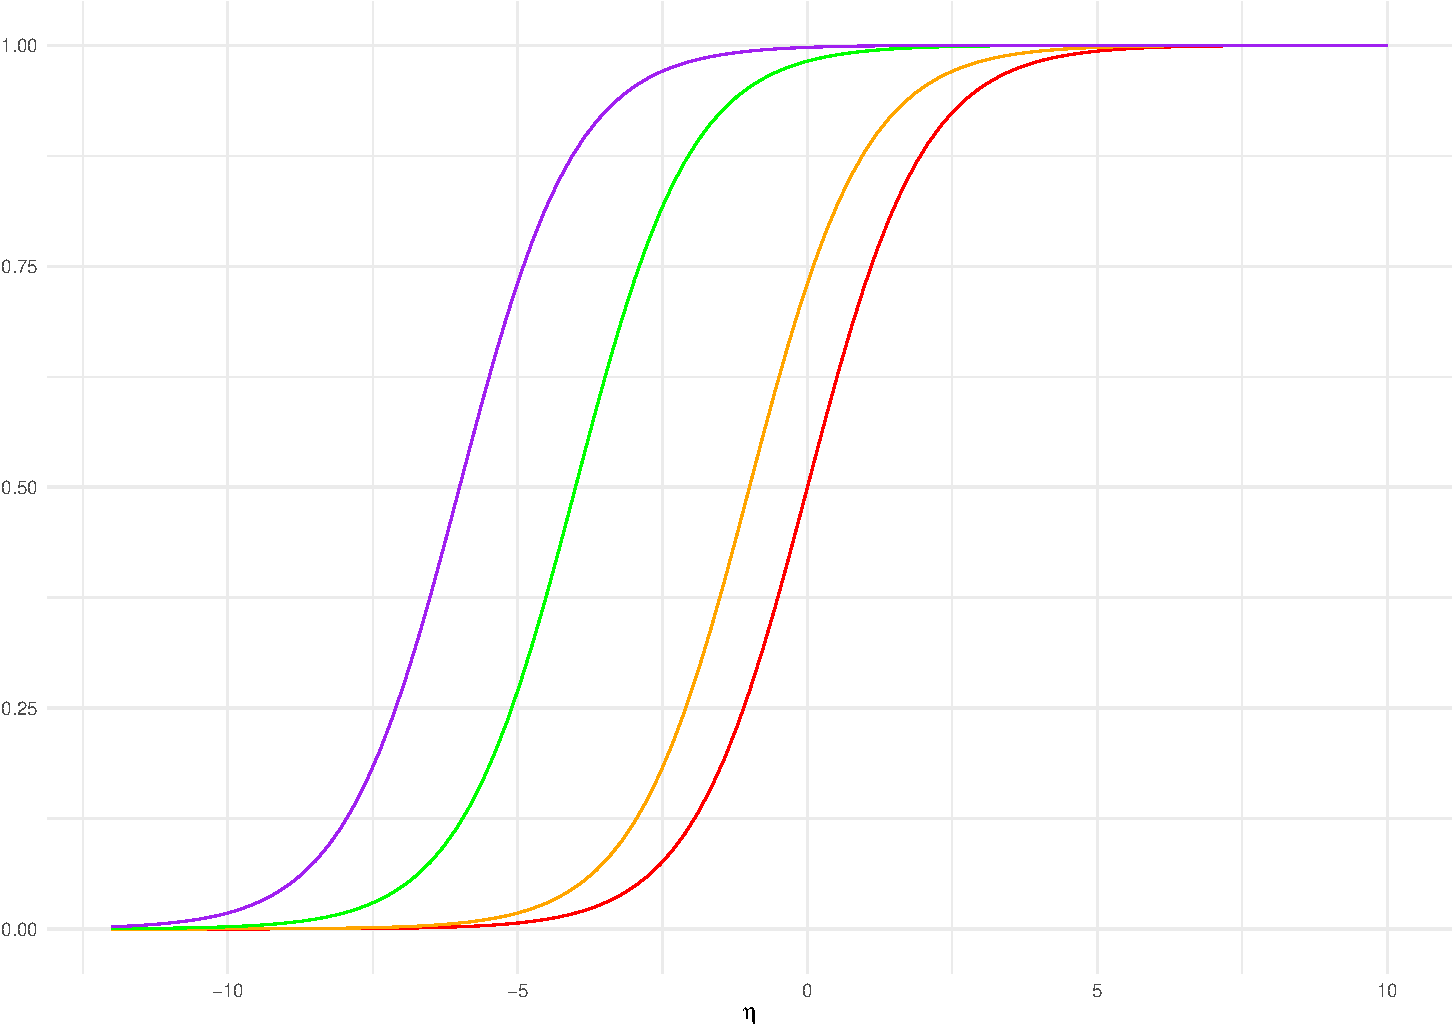
\includegraphics{Module06MultinomPresentation_files/figure-beamer/unnamed-chunk-9-1.pdf}
\end{frame}

\begin{frame}
\begin{block}{Mental health data example}
\protect\hypertarget{mental-health-data-example}{}
Example and data are taken from Agresti (2015, pages 219-223).

Research question: understand mental health issues.

The data comes from a random sample of size 40 of adult residents of
Alachua County, Florida, USA.

\begin{itemize}
\tightlist
\item
  Mental impairment \(Y\): 1=well, 2=mild symptom formation, 3=moderate
  symptom formation, 4=impaired.
\item
  Life event index (\(x_1\)): compsite measure of the number and
  severity of important life events within the last three years (birth,
  new job, divorce, death in the family, \ldots)
\item
  SES (\(x_2\)): socioeconomic index, 1=high, 0=low.
\end{itemize}

These data are ungrouped (but could be grouped). In the original study
several other explanatory variables were studied.
\end{block}
\end{frame}

\begin{frame}[fragile]
\begin{Shaded}
\begin{Highlighting}[]
\CommentTok{\# Read mental health data from the web:}
\FunctionTok{library}\NormalTok{(knitr)}
\NormalTok{data }\OtherTok{=} \StringTok{"http://www.stat.ufl.edu/\textasciitilde{}aa/glm/data/Mental.dat"}
\NormalTok{mental }\OtherTok{=} \FunctionTok{read.table}\NormalTok{(data, }\AttributeTok{header =}\NormalTok{ T)}
\FunctionTok{colnames}\NormalTok{(mental)}
\FunctionTok{apply}\NormalTok{(mental, }\DecValTok{2}\NormalTok{, table)}
\CommentTok{\# kable(mental)}
\end{Highlighting}
\end{Shaded}

\begin{verbatim}
## [1] "impair" "ses"    "life"  
## $impair
## 
##  1  2  3  4 
## 12 12  7  9 
## 
## $ses
## 
##  0  1 
## 18 22 
## 
## $life
## 
## 0 1 2 3 4 5 6 7 8 9 
## 2 5 4 8 5 4 2 2 4 4
\end{verbatim}
\end{frame}

\begin{frame}[fragile]
\begin{Shaded}
\begin{Highlighting}[]
\FunctionTok{library}\NormalTok{(VGAM)}
\CommentTok{\# We fit a cumulative logit model with main effects of \textquotesingle{}ses\textquotesingle{} and \textquotesingle{}life\textquotesingle{}:}
\NormalTok{fit.imp }\OtherTok{=} \FunctionTok{vglm}\NormalTok{(impair }\SpecialCharTok{\textasciitilde{}}\NormalTok{ life }\SpecialCharTok{+}\NormalTok{ ses, }\AttributeTok{family =} \FunctionTok{cumulative}\NormalTok{(}\AttributeTok{parallel =}\NormalTok{ T), }\AttributeTok{data =}\NormalTok{ mental)}
\CommentTok{\# parallell=T gives proportional odds structure {-} only intercepts differ}
\FunctionTok{summary}\NormalTok{(fit.imp)}
\end{Highlighting}
\end{Shaded}

\begin{verbatim}
## 
## Call:
## vglm(formula = impair ~ life + ses, family = cumulative(parallel = T), 
##     data = mental)
## 
## Coefficients: 
##               Estimate Std. Error z value Pr(>|z|)   
## (Intercept):1  -0.2819     0.6231  -0.452  0.65096   
## (Intercept):2   1.2128     0.6511   1.863  0.06251 . 
## (Intercept):3   2.2094     0.7171   3.081  0.00206 **
## life           -0.3189     0.1194  -2.670  0.00759 **
## ses             1.1112     0.6143   1.809  0.07045 . 
## ---
## Signif. codes:  0 '***' 0.001 '**' 0.01 '*' 0.05 '.' 0.1 ' ' 1
## 
## Names of linear predictors: logitlink(P[Y<=1]), logitlink(P[Y<=2]), 
## logitlink(P[Y<=3])
## 
## Residual deviance: 99.0979 on 115 degrees of freedom
## 
## Log-likelihood: -49.5489 on 115 degrees of freedom
## 
## Number of Fisher scoring iterations: 5 
## 
## No Hauck-Donner effect found in any of the estimates
## 
## 
## Exponentiated coefficients:
##      life       ses 
## 0.7269742 3.0380707
\end{verbatim}
\end{frame}

\begin{frame}
The ML fit for this model can be written as

\[ \text{logit}(\hat{P}(y_i\le r))=\hat{\theta}_r+0.319 x_{i1}+1.111 x_{i2}\]

\textbf{Q}: give an interpretation of this model!

Remember:

\begin{itemize}
\tightlist
\item
  Life event index (\(x_1\)): compsite measure of the number and
  severity of important life events within the last three years (birth,
  new job, divorce, death in the family, \ldots)
\item
  SES (\(x_2\)): socioeconomic index, 1=high, 0=low.
\end{itemize}
\end{frame}

\begin{frame}[fragile]
\textbf{Q}: How can you interpret the last line below? Why is it
exp(CI(beta)) and not CI(exp(beta))?

\begin{Shaded}
\begin{Highlighting}[]
\FunctionTok{exp}\NormalTok{(}\FunctionTok{confint}\NormalTok{(fit.imp))}
\end{Highlighting}
\end{Shaded}

\begin{verbatim}
##                   2.5 %     97.5 %
## (Intercept):1 0.2224503  2.5581328
## (Intercept):2 0.9385968 12.0489557
## (Intercept):3 2.2342109 37.1467162
## life          0.5752574  0.9187045
## ses           0.9114465 10.1266209
\end{verbatim}
\end{frame}

\begin{frame}[fragile]
\textbf{Q}: How are these predictions calculated? What is the
interpretation?

\begin{Shaded}
\begin{Highlighting}[]
\NormalTok{fitted }\OtherTok{=} \FunctionTok{data.frame}\NormalTok{(}\FunctionTok{fitted}\NormalTok{(fit.imp), }\AttributeTok{ses =}\NormalTok{ mental}\SpecialCharTok{$}\NormalTok{ses, }\AttributeTok{life =}\NormalTok{ mental}\SpecialCharTok{$}\NormalTok{life)}
\NormalTok{fitted[}\FunctionTok{c}\NormalTok{(}\DecValTok{6}\NormalTok{, }\DecValTok{18}\NormalTok{, }\DecValTok{10}\NormalTok{), ]  }\CommentTok{\#0,7 not fitted}

\NormalTok{xs }\OtherTok{=} \FunctionTok{cbind}\NormalTok{(}\FunctionTok{c}\NormalTok{(}\DecValTok{2}\NormalTok{, }\DecValTok{7}\NormalTok{, }\DecValTok{2}\NormalTok{, }\DecValTok{7}\NormalTok{), }\FunctionTok{c}\NormalTok{(}\DecValTok{0}\NormalTok{, }\DecValTok{0}\NormalTok{, }\DecValTok{1}\NormalTok{, }\DecValTok{1}\NormalTok{))}
\NormalTok{coeff }\OtherTok{=} \FunctionTok{coefficients}\NormalTok{(fit.imp)}
\NormalTok{linpreds }\OtherTok{=} \FunctionTok{cbind}\NormalTok{(coeff[}\DecValTok{1}\NormalTok{] }\SpecialCharTok{+}\NormalTok{ xs }\SpecialCharTok{\%*\%}\NormalTok{ coeff[}\DecValTok{4}\SpecialCharTok{:}\DecValTok{5}\NormalTok{], coeff[}\DecValTok{2}\NormalTok{] }\SpecialCharTok{+}\NormalTok{ xs }\SpecialCharTok{\%*\%}\NormalTok{ coeff[}\DecValTok{4}\SpecialCharTok{:}\DecValTok{5}\NormalTok{], coeff[}\DecValTok{3}\NormalTok{] }\SpecialCharTok{+}
\NormalTok{    xs }\SpecialCharTok{\%*\%}\NormalTok{ coeff[}\DecValTok{4}\SpecialCharTok{:}\DecValTok{5}\NormalTok{])}
\NormalTok{(}\AttributeTok{cprobs =} \FunctionTok{exp}\NormalTok{(linpreds)}\SpecialCharTok{/}\NormalTok{(}\DecValTok{1} \SpecialCharTok{+} \FunctionTok{exp}\NormalTok{(linpreds)))}
\NormalTok{(}\AttributeTok{pprobs =} \FunctionTok{cbind}\NormalTok{(cprobs[, }\DecValTok{1}\NormalTok{], cprobs[, }\DecValTok{2}\NormalTok{] }\SpecialCharTok{{-}}\NormalTok{ cprobs[, }\DecValTok{1}\NormalTok{], cprobs[, }\DecValTok{3}\NormalTok{] }\SpecialCharTok{{-}}\NormalTok{ cprobs[, }\DecValTok{2}\NormalTok{],}
    \DecValTok{1} \SpecialCharTok{{-}}\NormalTok{ cprobs[, }\DecValTok{3}\NormalTok{]))}
\end{Highlighting}
\end{Shaded}

\begin{verbatim}
##           X1        X2         X3         X4 ses life
## 6  0.2850362 0.3548973 0.18808559 0.17198084   0    2
## 18 0.5477558 0.2959810 0.09227184 0.06399141   1    2
## 10 0.1973858 0.3255923 0.22513134 0.25189056   1    7
##            [,1]      [,2]      [,3]
## [1,] 0.28503623 0.6399336 0.8280192
## [2,] 0.07488691 0.2651744 0.4943332
## [3,] 0.54775576 0.8437368 0.9360086
## [4,] 0.19738576 0.5229781 0.7481094
##            [,1]      [,2]       [,3]       [,4]
## [1,] 0.28503623 0.3548973 0.18808559 0.17198084
## [2,] 0.07488691 0.1902875 0.22915882 0.50566678
## [3,] 0.54775576 0.2959810 0.09227184 0.06399141
## [4,] 0.19738576 0.3255923 0.22513134 0.25189056
\end{verbatim}
\end{frame}

\begin{frame}[fragile]
\textbf{Q}: What do you see here, and what is the formula for this
matrix?

\begin{Shaded}
\begin{Highlighting}[]
\FunctionTok{vcov}\NormalTok{(fit.imp)}
\end{Highlighting}
\end{Shaded}

\begin{verbatim}
##               (Intercept):1 (Intercept):2 (Intercept):3        life         ses
## (Intercept):1    0.38819709    0.32992954    0.32615019 -0.04231112 -0.15615761
## (Intercept):2    0.32992954    0.42395851    0.40844529 -0.05427393 -0.11440293
## (Intercept):3    0.32615019    0.40844529    0.51423495 -0.06185757 -0.09055667
## life            -0.04231112   -0.05427393   -0.06185757  0.01426291 -0.01855824
## ses             -0.15615761   -0.11440293   -0.09055667 -0.01855824  0.37732634
\end{verbatim}
\end{frame}

\begin{frame}[fragile]
\begin{Shaded}
\begin{Highlighting}[]
\CommentTok{\# We consider a model with interaction between \textquotesingle{}ses\textquotesingle{} and \textquotesingle{}life\textquotesingle{}:}
\NormalTok{fit.int }\OtherTok{=} \FunctionTok{vglm}\NormalTok{(impair }\SpecialCharTok{\textasciitilde{}}\NormalTok{ life }\SpecialCharTok{+}\NormalTok{ ses }\SpecialCharTok{+}\NormalTok{ life}\SpecialCharTok{:}\NormalTok{ses, }\AttributeTok{family =} \FunctionTok{cumulative}\NormalTok{(}\AttributeTok{parallel =}\NormalTok{ T),}
    \AttributeTok{data =}\NormalTok{ mental)}
\FunctionTok{summary}\NormalTok{(fit.int)}
\end{Highlighting}
\end{Shaded}

\begin{verbatim}
## 
## Call:
## vglm(formula = impair ~ life + ses + life:ses, family = cumulative(parallel = T), 
##     data = mental)
## 
## Coefficients: 
##               Estimate Std. Error z value Pr(>|z|)   
## (Intercept):1  0.09807    0.81102   0.121  0.90375   
## (Intercept):2  1.59248    0.83717   1.902  0.05714 . 
## (Intercept):3  2.60660    0.90966   2.865  0.00416 **
## life          -0.42045    0.19031  -2.209  0.02715 * 
## ses            0.37090    1.13022   0.328  0.74279   
## life:ses       0.18131    0.23611   0.768  0.44255   
## ---
## Signif. codes:  0 '***' 0.001 '**' 0.01 '*' 0.05 '.' 0.1 ' ' 1
## 
## Names of linear predictors: logitlink(P[Y<=1]), logitlink(P[Y<=2]), 
## logitlink(P[Y<=3])
## 
## Residual deviance: 98.5044 on 114 degrees of freedom
## 
## Log-likelihood: -49.2522 on 114 degrees of freedom
## 
## Number of Fisher scoring iterations: 5 
## 
## No Hauck-Donner effect found in any of the estimates
## 
## 
## Exponentiated coefficients:
##      life       ses  life:ses 
## 0.6567529 1.4490350 1.1987822
\end{verbatim}
\end{frame}

\begin{frame}[fragile]
\begin{Shaded}
\begin{Highlighting}[]
\CommentTok{\# And test if there is a significant effect of interaction:}
\NormalTok{G2 }\OtherTok{=} \FunctionTok{deviance}\NormalTok{(fit.imp) }\SpecialCharTok{{-}} \FunctionTok{deviance}\NormalTok{(fit.int)}
\NormalTok{df.diff }\OtherTok{=} \FunctionTok{df.residual}\NormalTok{(fit.imp) }\SpecialCharTok{{-}} \FunctionTok{df.residual}\NormalTok{(fit.int)}
\DecValTok{1} \SpecialCharTok{{-}} \FunctionTok{pchisq}\NormalTok{(G2, df.diff)}
\CommentTok{\# The effect of interaction is not significant}
\end{Highlighting}
\end{Shaded}

\begin{verbatim}
## [1] 0.4410848
\end{verbatim}

\begin{Shaded}
\begin{Highlighting}[]
\CommentTok{\# We consider a model where the effect of the covariates may differ between the}
\CommentTok{\# cumulative logits {-} so not parallell lines for the cdfs}
\NormalTok{fit.nopar }\OtherTok{=} \FunctionTok{vglm}\NormalTok{(impair }\SpecialCharTok{\textasciitilde{}}\NormalTok{ life }\SpecialCharTok{+}\NormalTok{ ses, }\AttributeTok{family =}\NormalTok{ cumulative, }\AttributeTok{data =}\NormalTok{ mental)}
\FunctionTok{summary}\NormalTok{(fit.nopar)}

\CommentTok{\# The change in the deviance compared to the model \textquotesingle{}fit.imp\textquotesingle{} is}
\CommentTok{\# 99.0979{-}96.7486=2.3493 with df.diff=115{-}111=4, which is not significant}

\CommentTok{\# So model \textquotesingle{}fit.imp\textquotesingle{}seems fine.}
\end{Highlighting}
\end{Shaded}

\begin{verbatim}
## 
## Call:
## vglm(formula = impair ~ life + ses, family = cumulative, data = mental)
## 
## Coefficients: 
##               Estimate Std. Error z value Pr(>|z|)  
## (Intercept):1  -0.1930     0.7387  -0.261   0.7938  
## (Intercept):2   0.8278     0.7036   1.176   0.2394  
## (Intercept):3   2.8049     0.9615      NA       NA  
## life:1         -0.3182     0.1597  -1.993   0.0463 *
## life:2         -0.2739     0.1372  -1.997   0.0458 *
## life:3         -0.3964     0.1592  -2.490   0.0128 *
## ses:1           0.9732     0.7720   1.261   0.2074  
## ses:2           1.4962     0.7460   2.006   0.0449 *
## ses:3           0.7518     0.8358   0.899   0.3684  
## ---
## Signif. codes:  0 '***' 0.001 '**' 0.01 '*' 0.05 '.' 0.1 ' ' 1
## 
## Names of linear predictors: logitlink(P[Y<=1]), logitlink(P[Y<=2]), 
## logitlink(P[Y<=3])
## 
## Residual deviance: 96.7486 on 111 degrees of freedom
## 
## Log-likelihood: -48.3743 on 111 degrees of freedom
## 
## Number of Fisher scoring iterations: 14 
## 
## Warning: Hauck-Donner effect detected in the following estimate(s):
## '(Intercept):3'
## 
## 
## Exponentiated coefficients:
##    life:1    life:2    life:3     ses:1     ses:2     ses:3 
## 0.7274592 0.7604194 0.6727572 2.6465169 4.4645713 2.1207587
\end{verbatim}
\end{frame}

\begin{frame}
\begin{block}{Why not use MLR instead of ordinal regression?}
\protect\hypertarget{why-not-use-mlr-instead-of-ordinal-regression}{}
Based on Agresti (2015, p 214-216)

To use MLR the ordinal categories need to be replaced with numerical
values, and we then need to assume a normal error structure. The
following are questions to be answered and possible limitation to be
assumed for using MLR instead of ordinal regression:

\begin{itemize}
\tightlist
\item
  how to translate ordered categories into numerical scores?
\item
  is it better with an ordinal variable with some range than a single
  numerical number?
\item
  MLR will not give probabilities for each response category
\item
  variability in the response may be dependent on the category, for MLR
  we assume homoscedasticity
\end{itemize}
\end{block}
\end{frame}

\begin{frame}{Likelihood inference}
\protect\hypertarget{likelihood-inference}{}
We use the notation that \({\boldsymbol \beta}\) is a long vector with
all regression parameters. The content of this vector is slightly
different for our two models, with intercept and \(k\) covariate effects
for each response category for the nominal model - and with \(c\)
thresholds but the same \(k\)-dimensional \({\boldsymbol \beta}\) vector
for all categories.

Full matrix versions (over all \(i\)) can be found in our textbook, page
345-346.

\begin{block}{Loglikelihood}
\protect\hypertarget{loglikelihood-1}{}
We have seen that the loglikelihood is:
\[ l({\boldsymbol \beta})\propto\sum_{i=1}^n \sum_{s=1}^{c+1} y_{is}\ln(\pi_{is})\]

where we remember that \(y_{i,c+1}=n_i-y_{i1}-\cdots-y_{ic}\), and
\(1-\pi_{i1}-\cdots \pi_{ic}\).
\end{block}
\end{frame}

\begin{frame}
\begin{block}{Design matrix and coefficient vector}
\protect\hypertarget{design-matrix-and-coefficient-vector}{}
The design matrix \({\bf X}\) and coefficient vector are different for
our nominal logit model and our ordinal cumulative model.

\begin{block}{Nominal logit model}
\protect\hypertarget{nominal-logit-model}{}
\[{\bf X}_i=\text{diag}({\bf x}_i^T)=\begin{pmatrix}{\bf x}_i^T & 0 & \cdots & 0\\
0 & {\bf x}_i^T  & \cdots & 0\\
\vdots & \vdots & \ddots & \vdots\\
0 & 0 & \cdots & {\bf x}_i^T\\
\end{pmatrix}\]

where the \(0\)s are \(1\times p\) vectors. The dimension of the design
matrix for covariate pattern \(i\) is \(c \times c\cdot p\).
\end{block}
\end{block}
\end{frame}

\begin{frame}
The vector of coefficients has dimension \(c\cdot p \times 1\).
\[{\boldsymbol \beta}=\begin{pmatrix}{\boldsymbol \beta}_1\\{\boldsymbol \beta}_2\\\vdots\\{\boldsymbol \beta}_c\\ \end{pmatrix}\]
\end{frame}

\begin{frame}
\begin{block}{Ordinal cumulative model}
\protect\hypertarget{ordinal-cumulative-model}{}
\[{\bf X}_i=\begin{pmatrix}1 & 0 & \cdots & 0 & {\bf x}_i^T\\
0 & 1 & \cdots & 0 & {\bf x}_i^T\\
\vdots & \vdots & \ddots & \vdots \\
0 & 0 & \cdots & 1 & {\bf x}_i^T\\
\end{pmatrix}\] he dimension of the design matrix for covariate pattern
\(i\) is \(c \times (c+k)\)

The vector of coefficients has dimension \((c+ k) \times 1\) (where
\(p=k+1\)), and now the thresholds replace the intercept and are put
first in the vector, and the effects of the covariates are the same for
all categories.
\[{\boldsymbol \beta}=\begin{pmatrix}\theta_1\\ \theta_2 \\ \vdots \\ \theta_c \\{\boldsymbol \beta}\\ \end{pmatrix}\]
\end{block}
\end{frame}

\begin{frame}
\begin{block}{Score function}
\protect\hypertarget{score-function}{}
\[{\bf s}({\boldsymbol \beta})=\sum_{i=1}^G {\bf X}_i^T {\bf D}_i {\boldsymbol \Sigma}_i^{-1}({\bf y}_i-n_i{\boldsymbol \pi}_i)\]

where

\begin{itemize}
\tightlist
\item
  \({\bf D}_i=\frac{\partial {\boldsymbol h}({\boldsymbol \eta})}{\partial {\boldsymbol \eta}}\lvert_{{\boldsymbol \eta}={\boldsymbol \eta}_i}\)
  has dimension \(c \times c\)
\item
  \({\boldsymbol \Sigma}_i=\text{Cov}({\bf Y}_i)\)
\end{itemize}
\end{block}
\end{frame}

\begin{frame}
\begin{block}{Fisher information}
\protect\hypertarget{fisher-information}{}
The dimension of the matrix is \(cp\times cp\) for the nominal case and
\((c+k) \times (c+k)\) for the ordinal case studied.

\[F({\boldsymbol \beta})=\sum_{i=1}^G {\bf X}_i^T {\bf W}_i {\bf X}_i\]

where \({\bf W}_i\) is given as
\({\bf D}_i{\boldsymbol \Sigma}_i^{-1}{\bf D}_i^T\).
\end{block}
\end{frame}

\begin{frame}
\begin{block}{Finding the ML estimate}
\protect\hypertarget{finding-the-ml-estimate}{}
As in modules 1-5 we find the ML estimate by the Fisher scoring or
Newton Raphson method.
\end{block}

\begin{block}{Asymptotic distribution}
\protect\hypertarget{asymptotic-distribution}{}
As in modules 1-5 the ML estimator \(\hat{\boldsymbol \beta}\)
asymptotically follows a multivariate normal distribution with unbiased
mean and covariance matrix given by the inverse of the expected Fisher
information matrix.
\end{block}
\end{frame}

\begin{frame}{Summing up}
\protect\hypertarget{summing-up}{}
\end{frame}

\begin{frame}[fragile]{R packages}
\protect\hypertarget{r-packages}{}
\begin{Shaded}
\begin{Highlighting}[]
\FunctionTok{install.packages}\NormalTok{(}\FunctionTok{c}\NormalTok{(}\StringTok{"VGAM"}\NormalTok{, }\StringTok{"ggplot2"}\NormalTok{, }\StringTok{"statmod"}\NormalTok{, }\StringTok{"knitr"}\NormalTok{))}
\end{Highlighting}
\end{Shaded}
\end{frame}

\begin{frame}{Further reading}
\protect\hypertarget{further-reading}{}
\begin{itemize}
\tightlist
\item
  A. Agresti (2015): ``Foundations of Linear and Generalized Linear
  Models.'' Chapter 6. Wiley.
\end{itemize}
\end{frame}

\end{document}
